\documentclass{article}
\usepackage{a4wide}


\usepackage{polski}
\usepackage[utf8x]{inputenc}
\usepackage{graphicx}
\usepackage{float}
\usepackage{hyperref}
\usepackage{listings}
\usepackage{mathtools}
\usepackage{amsmath}

\usepackage{color} %red, green, blue, yellow, cyan, magenta, black, white
\definecolor{mygreen}{RGB}{28,172,0} % color values Red, Green, Blue
\definecolor{taupe}{rgb}{0.28, 0.24, 0.2}
\definecolor{mylilas}{RGB}{0,110,0}


\author{Lev Sergeyev}
\title{SPC. Ćwiczenie 2. Charakterystyki częstotliwościowe. \\ Sprawozdanie}

\date{25.10.2019, pt/TN 13:15}
\begin{document}

\maketitle

%\pagebreak


\section{Charakterystyka amplitudowo-fazowa}
\par
Dany układ o transmitancji:
\begin{equation}
K(s)=\frac{ke^{-s\tau}}{Ts+1} 
\end{equation}
Przekształcono ukłąd na postać \( K(j\omega)\), podzielono na część urojoną i rzeczywistą (3) aby utworzyć chrakterystykę amplitudowo-fazową (Rys. 1)

\begin{equation}
K(j\omega)=
\frac{k(\cos(-\omega\tau)+j\sin(-\omega\tau)}{T j\omega+1}=
-\frac{T\omega k \sin(\omega\tau) -k \cos(\omega\tau)}{T^2\omega^2+1}
-j\frac{T\omega k \cos(\omega\tau) -k \sin(\omega\tau)}{T^2\omega^2+1}
\end{equation}


Na charakterystyce wybrano dwa punkty, dla róźnych \(\omega\).
Dla danego układu o dobranych \(k, \tau\) i \(T\) jak na Rys. 1 kąt przesunięcia \(\phi\) rośnie a wzmocnienie \(A\) maleje wraz z wzrostem \(\omega\).

\begin{figure}[h]
\centering
\scalebox{0.3}{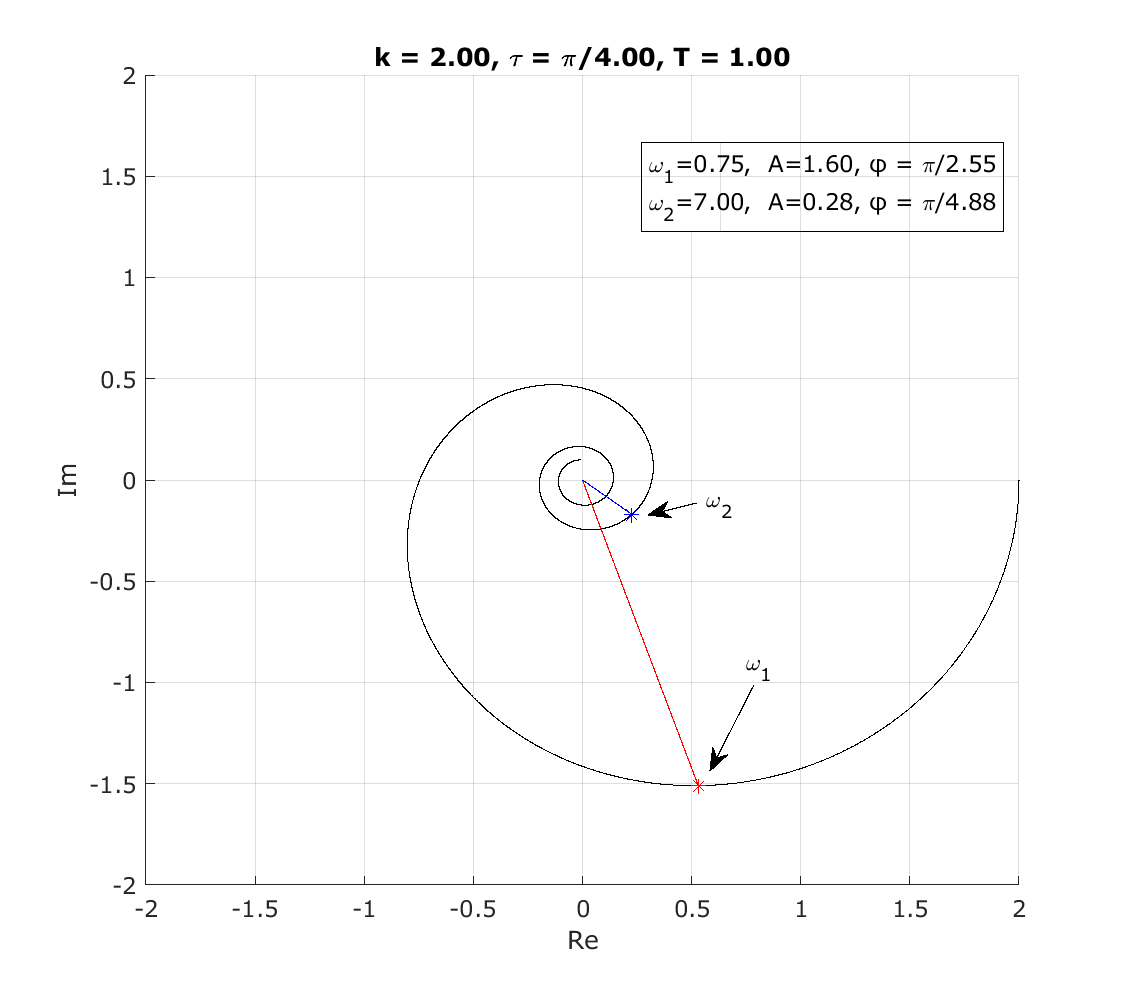
\includegraphics{freq.png}}
\caption{Charakterystyka Nyquista dla K(s)}
\end{figure}


%\pagebreak

\section{Odpowiedź układu na wymuszenie}

Sprawdzono, czy otrzymana charakterystyka rzeczywiście zachodzi dla \( \omega_1\) i \(\omega_2 \), podanego układu i jego parametrów \(k, \tau, T\).
Za pomocą modelu simulink w którym część układu \(e^{-s\tau}\) zastąpiono bloczkiem przesunięcia, przeprowadzono symulację odpowiedzi, kiedy na wejściu jest sygnał \(u(t)=\sin(\omega t)\), z wybranymi z poprzedniego rozdziału \( \omega_1\) i \(\omega_2 \):


\begin{figure}[h]
\centering
\scalebox{0.2}{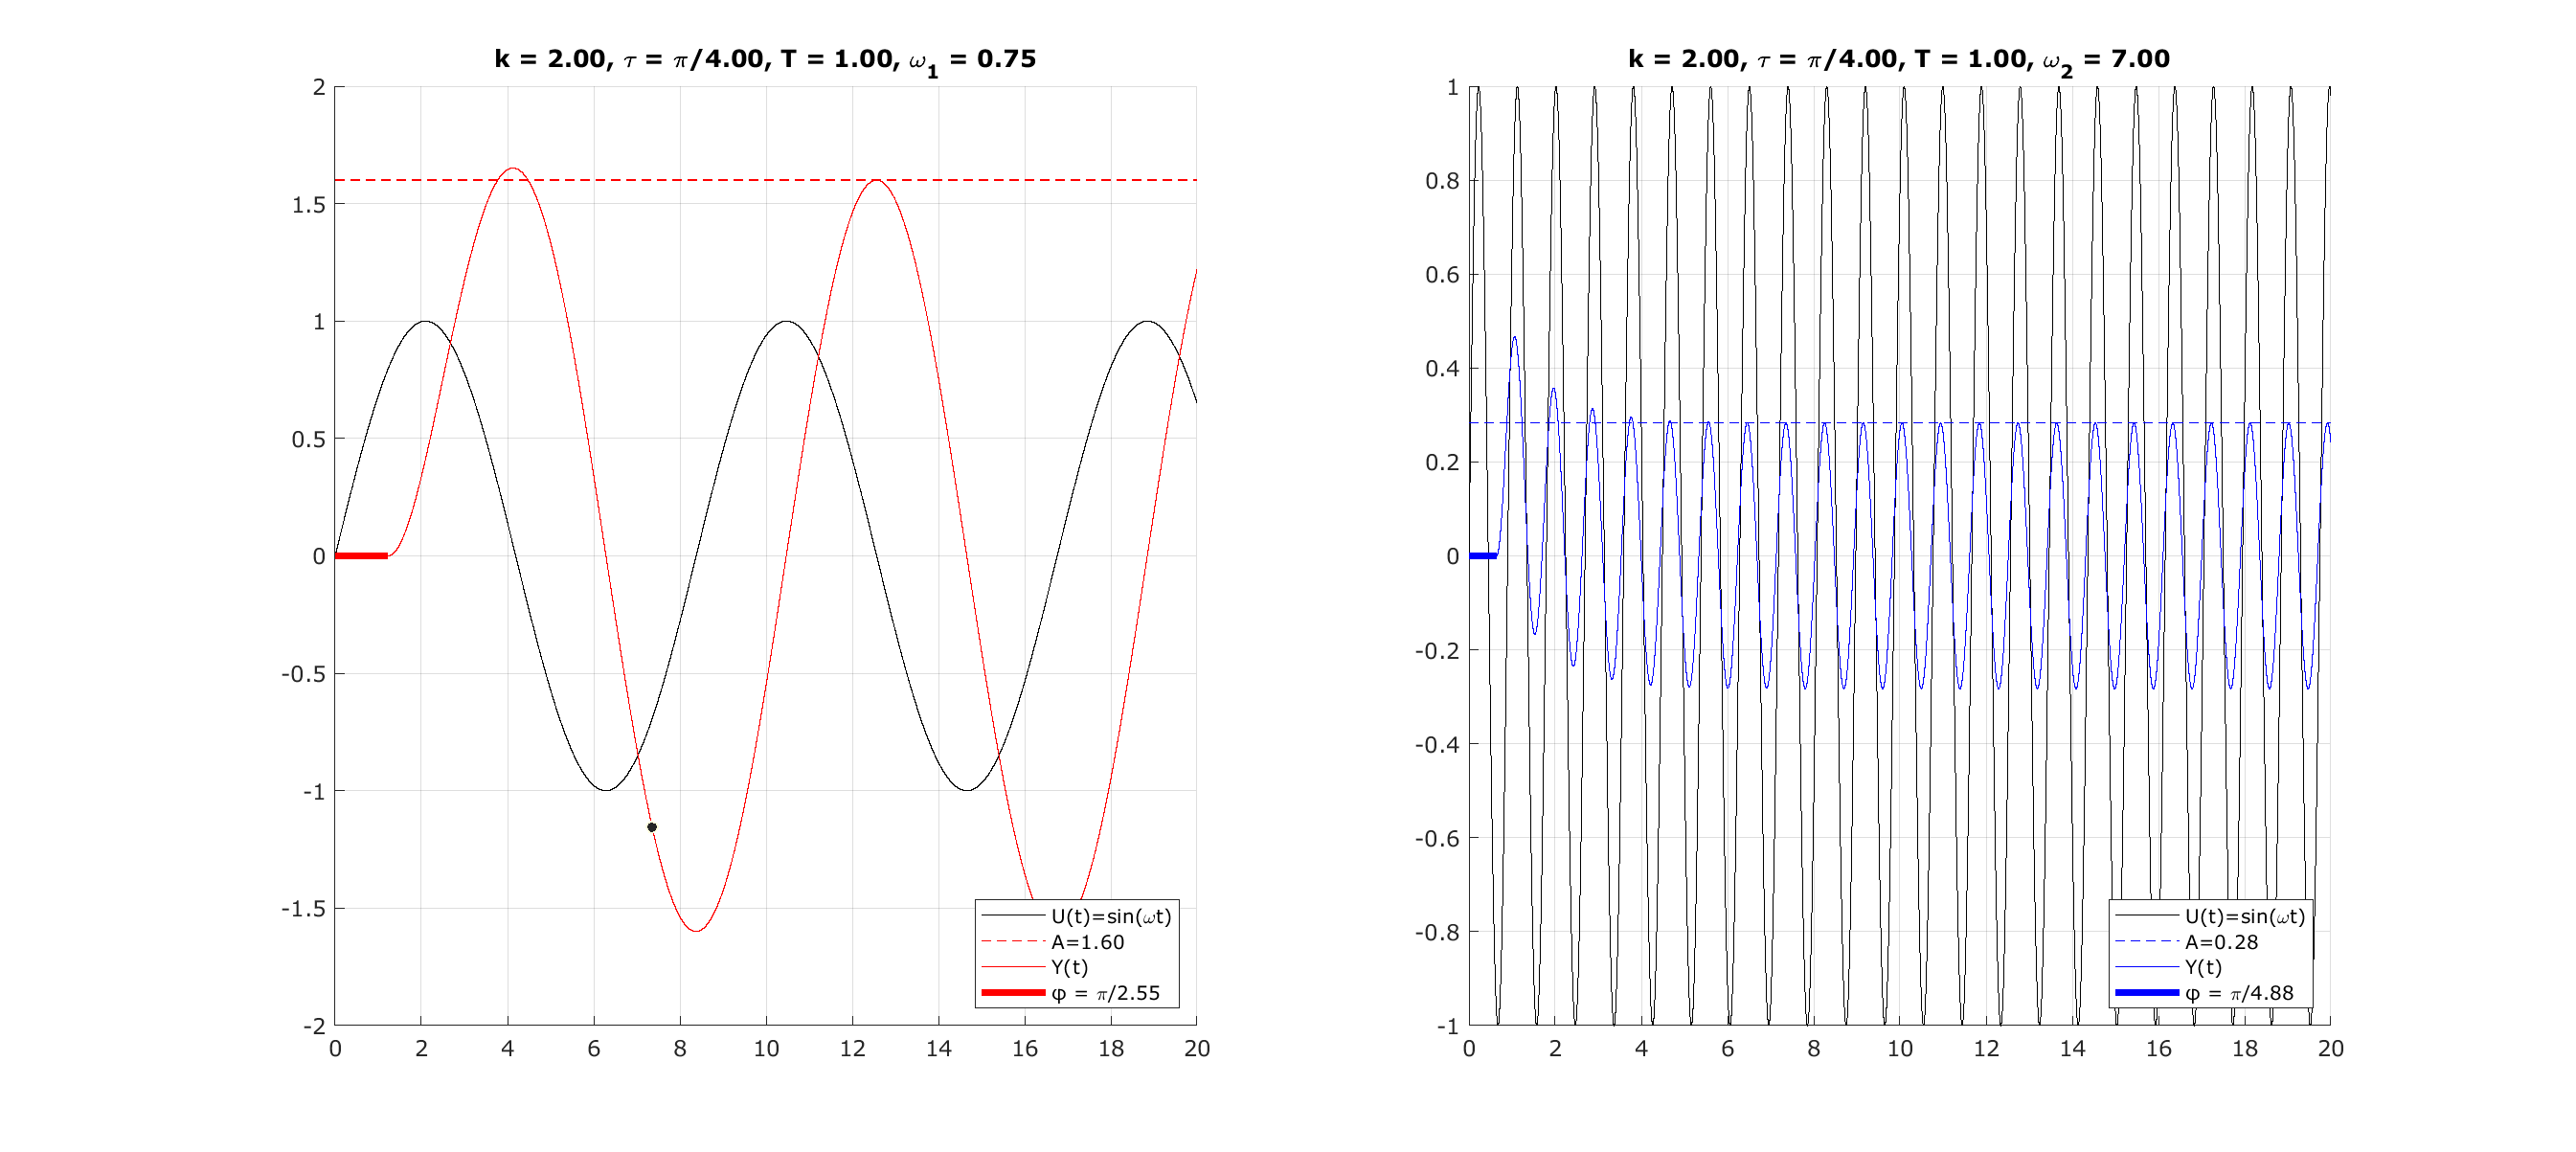
\includegraphics{sin.png}}
\caption{Odpowiedź układu \( K(s) \) na wymuszenie \(u(t)=\sin(\omega t)\)}
\end{figure}

\section{Wnioski}

Wykres odzyskanej odpowiedzi (Rys. 2) udowadnia to, że przesunięcie \(\phi\) i wzmocnienie \(A\) wyznaczone na charakterystyce amplitudowo-fazowej  rzeczywiście są takie same dla odpowiedzi na sygnał \(u(t)=\sin(\omega t)\) dla wybranych pulsacji \( \omega_1\) i \(\omega_2 \). Zniekształcenia na początku odpowiedzi mogą się pojawiać przez opóźnienie przejścia systemu z stanu ustalonego na stan pobudzenia sygnałem wejściowym.



\end{document}
